\chapter{Merging algorithm}

In this chapter we present an merging algorithm based on computer vision techniques. This is not completely new even in ROS environment. First computer vision-based approach to merging was implemented in \cite{MapstitchROS}. This package's primary purpose was to stitch generated map to existing static map.

Although this package was not developed for map merging in multi-robot configuration, algorithm and its original implementation were used for coordinated multi-robot exploration solution presented in \cite{Andre2014}.

Due to its original purpose, mapstitch algorithm shows some limitations for multi-robot map merging setup. Originally it was designed for offline use \cite{Andre2014}. Also, it was designed for stitching two maps, one them being large reference map covering most of the environment. Although it is possible to incrementally merge maps from multiple robots with this algorithm, global map quality generally decreases with increasing number of robots. \cite{Andre2014}. Significant decrease in performance was observed for 4 robots\cite{Andre2014}.

\begin{algorithm}
    \caption{Mapstitch original algorithm}
    \label{alg:mapstitch}
    \begin{algorithmic}[1]
        \Procedure{StitchedMap}{$grid1, grid2$}
            \State detect Orb features
            \State match keypoints with Brute-Force matcher
            \State find matching point pairs with same distance in both images
            \State find homography (affine transform)
        \EndProcedure
    \end{algorithmic}
\end{algorithm}

Algorithm~\ref{alg:mapstitch} shows original algorithm used in \cite{MapstitchROS}, version used in \cite{Andre2014} is only a slightly modified.

Although our algorithm also uses computer vision-based approach, proposed algorithm deals with most of the limitations of the original simple algorithm. Proposed algorithm is designed to work with unlimited number of grids, so it requires no additional need for iterative merging. More importantly, by design, algorithm can determine optimal order of individual pairwise merges. I assume this might be the main reason for decrease in performance in $4$-robot setup observed by\cite{Andre2014}. Also proposed algorithm deals with other problems arising for general $n$-map merge problem such as situations when it is not possible to merge some of the maps because transformation to others could not be reliably estimated, cases where map transformation can be estimated from more sources (multiple neighbours) etc.

\section{Stitching pipeline}

As discussed in chapter \#reference here\# our algorithm is inspired by image stitching algorithms. Stitching algorithms are well-understood and implementations are broadly available. General concept of multi-step stitching pipeline is described in \cite{Brown2006}. Stitching pipeline is also well established code in OpenCV, mostly based on \cite{Brown2006}, along with \cite{Szeliski2004} \cite{Shum1998} and others. Figure~\ref{fig:opencv} highlights processing steps in stitching as implemented in OpenCV.

\begin{figure}
	\centering
	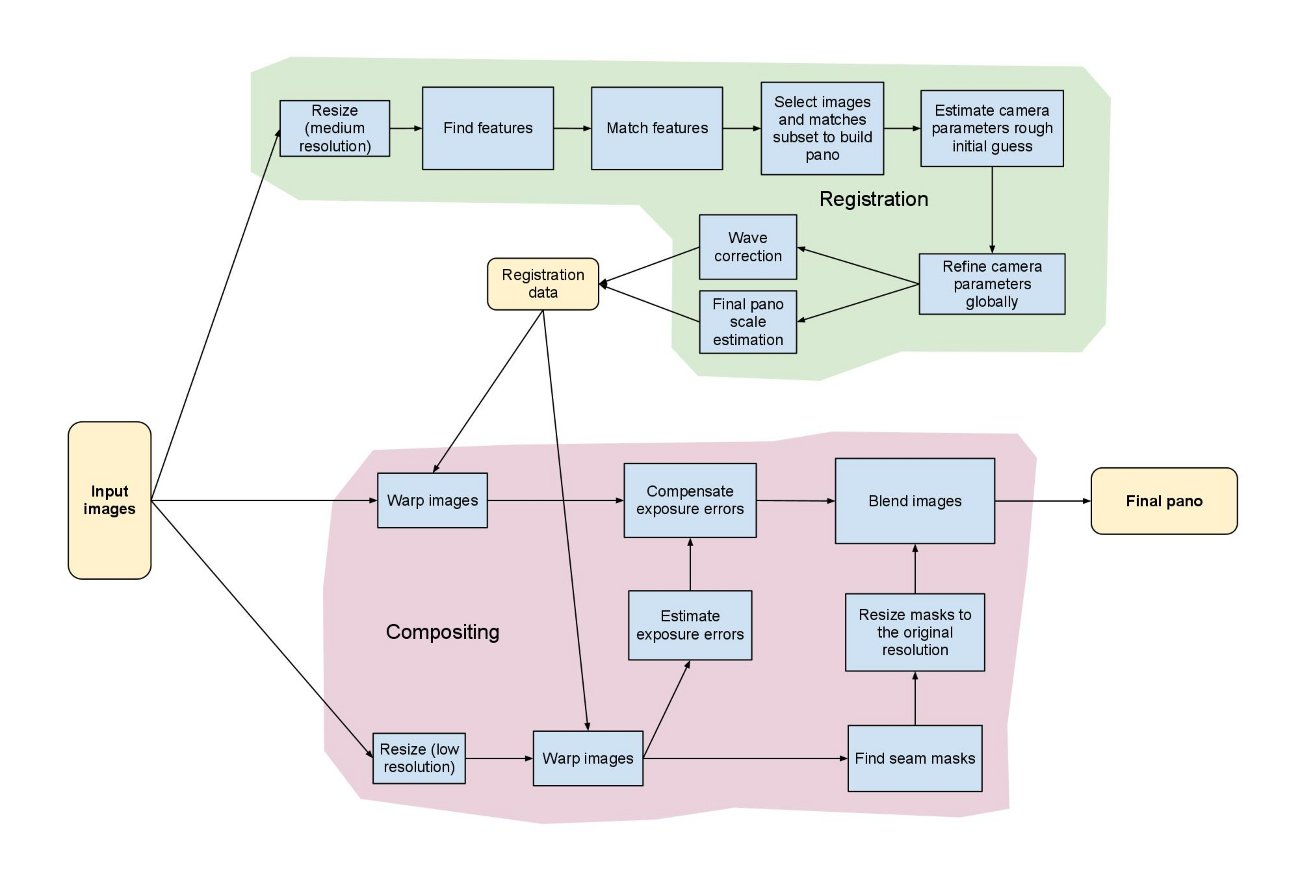
\includegraphics[width=4.33in]{../img/StitchingPipeline.jpg}
	\caption{OpenCV Stitching pipeline.}
	\label{fig:opencv}
\end{figure}

Our algorithm will solve the registration part of stitching according to figure~\ref{fig:opencv}. As compositing part of stitching is relatively simple for occupancy grids compared to images from camera, this solves the main problem of acquiring transformation between robots individual frames and bridging the problem of merging maps with known initial positions and unknown initial positions.

ROS node for map merging described in \#reference here\# implements also compositing part of the pipeline, which is simple when transformation is estimated with high precision.

For description of the algorithm we will assume to have maps represented as occupancy grids, with each cell containing value in range $[0,100]$ indicating probability that there is obstacle in the cell and $-1$ for indicating unknown probability. This representation is basically greyscale image, hence using image processing algorithms seems natural.

We will with occupancy grids as greyscale images through algorithm~\ref{alg:estimategridtrasform}. Values in the image are exactly the same is in occupancy grids, without any mapping. This means images are be basically only $7$-bit depth.

Algorithm~\ref{alg:estimategridtrasform} offers overview of the proposed algorithm, detailed description will be provided in following sections.

\begin{algorithm}
    \caption{Proposed algorithm for estimating transform between multiple occupancy grids}
    \label{alg:estimategridtrasform}
    \begin{algorithmic}[1]
        \Procedure{estimateGridTransform}{$grids$}
            \State detect Orb features (keypoints) for each grid
            \ForAll{pair of grids} \Comment{we will compute transformation between each image along with confidence}
            	\State match features
            	\State $n \gets \text{number of matches}$
            	\If{$n \le $}
            		\State confidence $\gets 0$
            	\Else
            		\State find restricted affine transformation for keypoints using RANSAC
            		\State $\vartheta \gets \text{number of inliers in RANSAC}$
            		\If{transformation found}
            			\State confidence $\gets \frac{\vartheta}{8 + 0.3 \cdot n}$
            		\Else
            			\State confidence $\gets 0$
            		\EndIf
            	\EndIf
            \EndFor
            \State matches $\gets (i,j)$ for matches with confidence $\ge 1.0$
            \State $g \gets (grids, matches)$
            \State $h \gets$ largest connected component in $g$
            \State $t \gets$ maximum spanning tree in $h$
            \State walk $t$ and compute transformations to global reference frame
        \EndProcedure
    \end{algorithmic}
\end{algorithm}